% coding:utf-8

%----------------------------------------
%FOSAPHY, a LaTeX-Code for a summary of modern control theory
%Copyright (C) 2015, Mario Felder & Michi Fallegger

%This program is free software; you can redistribute it and/or
%modify it under the terms of the GNU General Public License
%as published by the Free Software Foundation; either version 2
%of the License, or (at your option) any later version.

%This program is distributed in the hope that it will be useful,
%but WITHOUT ANY WARRANTY; without even the implied warranty of
%MERCHANTABILITY or FITNESS FOR A PARTICULAR PURPOSE.  See the
%GNU General Public License for more details.
%----------------------------------------

\section{Regelungsnormalform der Zustandsgleichung}
\[
	Y(s) = G(s) \cdot U(s)
\]
\[
	G(s)= \frac{Z(s)}{N(s)} = \frac{b_0+b_1s+b_2s^2+...+b_ns^n}{a_0+a_1s+a_2s^2+...+a_ns^n}=c\cdot(sI-A)^{-1}\cdot B +D
\]
\subsection{Signalflussbild}
\begin{center}
	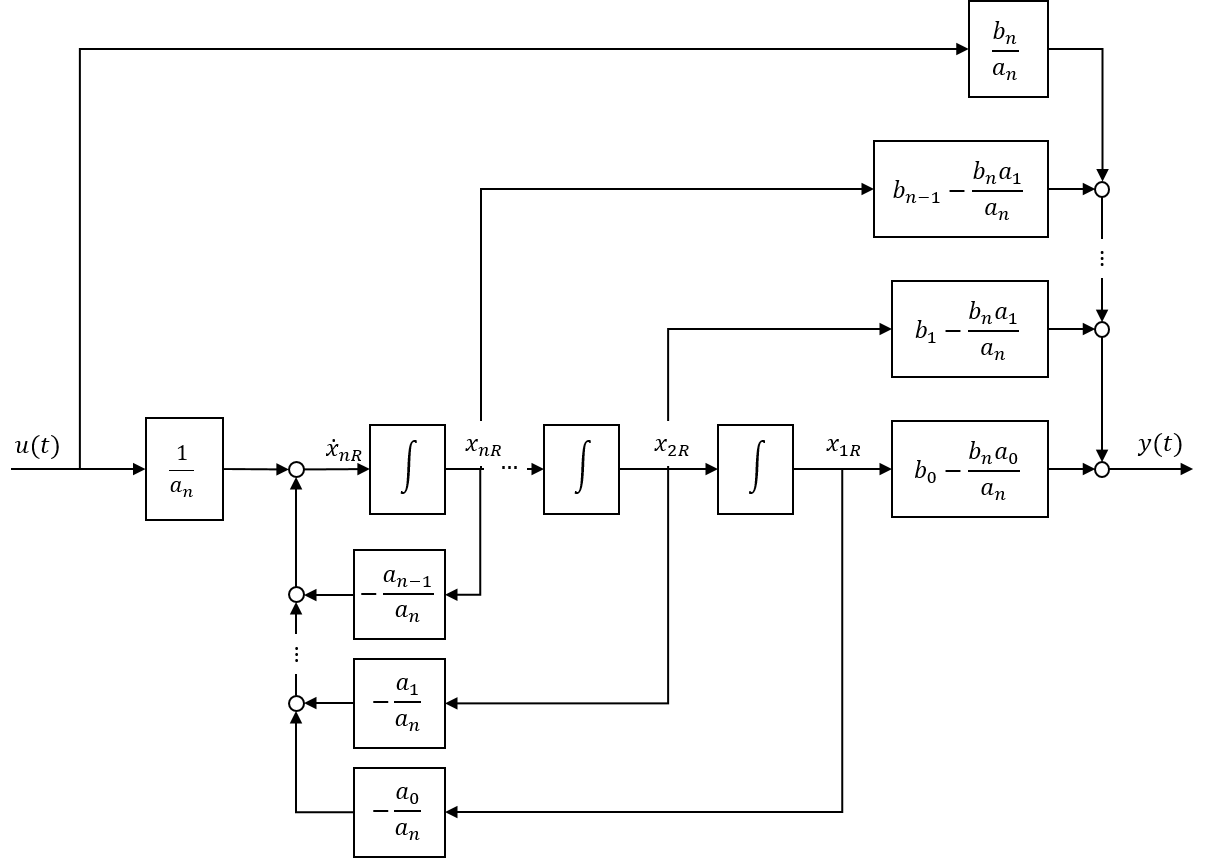
\includegraphics[scale = 0.5]{images/RNF_Signalflussblid.png}
\end{center}

\subsection{Regelungsnormalform}
\[
	\dot x=
	\underbrace{
		\begin{bmatrix}
			0 &	1 & 0 & \ldots & 0\\
			0 & 0 & 1 & \ldots & 0\\
			\vdots & \vdots & \vdots & \ddots & \vdots \\
			0 & 0 & 0 & \ldots & 1\\
			-\frac{a_0}{a_n} &-\frac{a_1}{a_n} & -\frac{a_2}{a_n} & \ldots &-\frac{a_{n-1}}{a_n}\\	
		\end{bmatrix}
	}_{\textbf{A}}
	\cdot x +
	\underbrace{
		\begin{bmatrix}
			0 \\
			0 \\
			\vdots \\
			0 \\
			\frac{1}{a_n} \\	
		\end{bmatrix}
	}_{\textbf{b}}
	\cdot u	
\]

\[
	y=
	\underbrace{
			\begin{bmatrix}
				b_0-a_0\cdot\frac{b_n}{a_n} & b_1-a_1\cdot\frac{b_n}{a_n} & \ldots & b_{n-1}-a_{n-1}\cdot\frac{b_n}{a_n} &\\
			\end{bmatrix}
	}_{\textbf{$c^T$}}
	\cdot x  +
	\underbrace{
		\left[ \frac{b_n}{a_n} \right] 
	}_{\textbf{d}}
	\cdot u
\]